% Created with jtex v.1.0.20
\documentclass{article}
\PassOptionsToPackage{short, nodayofweek}{datetime}


% Start Curvenote Definitions

% Pass Options Section
% base
\PassOptionsToPackage{normalem}{ulem}
\PassOptionsToPackage{utf8}{inputenc}

% template
\PassOptionsToPackage{framemethod=TikZ}{mdframed}
\PassOptionsToPackage{x11names, svgnames}{xcolor}

%%% PACKAGES

% base
\usepackage{inputenc}
\usepackage{url}
\usepackage{graphicx}
\usepackage{adjustbox}
\usepackage{amssymb}
\usepackage{amsfonts}
\usepackage{amsmath}
\usepackage{enumitem}
\usepackage{nicefrac}
\usepackage{booktabs}
\usepackage{microtype}
\usepackage{hyperref}
\usepackage{ulem}
\usepackage{enumitem}
\usepackage{float}
\usepackage{datetime}
\usepackage{xkeyval}
\usepackage{framed}
\usepackage{doi}

% template
\usepackage{natbib}
\usepackage{fancyvrb}
\usepackage{mdframed}
\usepackage{xcolor}

%%%


%%%% Setup Section

% base
\graphicspath{{.}}
% template
\sloppy
\newenvironment{aside}{\begin{framed}}{\end{framed}}
\newmdenv[linewidth=2pt,linecolor=CornflowerBlue,topline=false,bottomline=false,rightline=false,leftline=true,skipabove=20,skipbelow=20,leftmargin=20,rightmargin=20]{callout}
\newfloat{code}{thp}{loc}
\floatname{code}{Program}
\raggedbottom
\bibliographystyle{abbrvnat}
\setcitestyle{authoryear,open={(},close={)},semicolon,aysep={,}}

% End Curvenote Definitions




% colors for hyperlinks
\hypersetup{colorlinks=true, allcolors=blue}
\hypersetup{
pdftitle={\@title},
pdfsubject={},
pdfauthor={\@author},
pdfkeywords={},
addtopdfcreator={Written in Curvenote}
}

\usepackage{curvenote}

\title{Ch. 6: Dual EMG recordings of muscle pairs}

\newdate{articleDate}{3}{5}{2025}
\date{\displaydate{articleDate}}

\author{\bfseries Erin McKiernan\mdseries\\Universidad Nacional Autónoma de México (UNAM), Open Research Community Accelerator (ORCA)\\\AND\bfseries Saúl A. Saldaña Enciso\mdseries\\}

\begin{document}

\maketitle
\keywords{}

\section{Overview}

In this experimental practical, students learn how agonist-antagonist muscle pairs work to produce opposing movements like flexion and extension. Students learn how to record electromyograms (EMGs) from various of these muscle pairs and what types of movements activate them. Overall, this practical is designed to help students gain deeper understanding of the biomechanics of the musculoskeletal system, and how movement is related to electrical activity in groups of muscles. The duration of the practical can be as short as 30 minutes or up to 2 hours, depending on the number of muscle pairs recorded and the complexity of the different muscle activities explored. While not necessary, it is recommended that students carry out the experimental practical in \href{https://curvenote.com/oxa:EPpXta8zJdzN048lz8AR/hZTnTYzQR5EQmCKX51Wj}{Ch. 1: Muscle physiology and EMG basics }prior to this practical.

\section{Learning objectives}

\textbf{Before} this practical, students should be able to:

\begin{itemize}
\item understand the basics of muscle contraction, including how muscles contract and relax
\item explain the basics of EMG recording and how it is used to monitor muscle activity
\item identify different muscles within the human body that have opposing actions
\end{itemize}

\textbf{During} this practical, students will:

\begin{itemize}
\item learn how to record EMGs from agonist-antagonist muscle pairs, including proper electrode placement
\item observe and record changes in muscle activity during flexion and extension, or other opposing actions
\item compare and contrast recordings from different muscle pairs
\end{itemize}

\textbf{After} this practical, students should be able to:

\begin{itemize}
\item describe the actions of different muscle pairs and their importance for movements like walking
\item visually interpret dual EMG recordings from muscle pairs
\item design further experiments to record from additional muscle pairs, or explore under what movement conditions an agonist becomes an antagonist and vice versa
\end{itemize}

\section{Equipment and materials}

\begin{itemize}
\item EMG recording equipment, either:\begin{itemize}
\item 2x \href{https://backyardbrains.com/products/muscle-spikerbox}{Muscle SpikerBox} (Backyard Brains), one for each muscle channel; will need to have some way to synchronize the recordings, e.g. event markers, or
\item \href{https://backyardbrains.com/products/human-spikerbox}{Human SpikerBox} (Backyard Brains), which has built-in dual recording channels
\end{itemize}


\item 9V battery to power SpikerBox
\item Round surface electrodes (any medical supply provider)
\item Smaller tab electrodes that can be cut for smaller muscles like those in the hand (any provider)
\item Cables with alligator clips to connect electrodes to SpikerBox (Backyard Brains)
\item Cable to connect SpikerBox to a computer, tablet, or smartphone (Backyard Brains)
\item Computer, tablet, or phone with free Backyard Brains \href{https://backyardbrains.com/products/byb-spike-recorder}{Spike Recorder software} installed
\item Phone or tablet adaptor, 3.5mm aux to USB-C (if no aux port on devices; any provider)
\item Alcohol and cotton swabs to help remove electrodes after recording (optional)
\item Barbell or other weights to activate muscles (optional; can also do with just body weight)
\item Other indications: Wear loose clothing to permit electrode placement
\end{itemize}

\section{Background}

\subsection{Joints of the human body}

A joint is a specialized structure where two bones meet \citep{levangie2011joint}. If we think back to \href{https://curvenote.com/oxa:EPpXta8zJdzN048lz8AR/hZTnTYzQR5EQmCKX51Wj}{Ch. 1: Muscle physiology and EMG basics}, joints act as fulcrums or pivot points around which movement occurs. Synovial joints, in which the bones are separated by a space within a joint capsule filled with special fluid, allow for the greatest motility, and are the most prevalent type of joint found in the human body \citep{openStax_joints}. Synovial joints are further classified based on the shape of the bones, the form of their union, and the types of movement possible based on these factors \citep{}Figure \%s `` .

\begin{figure}[!htbp]
\centering
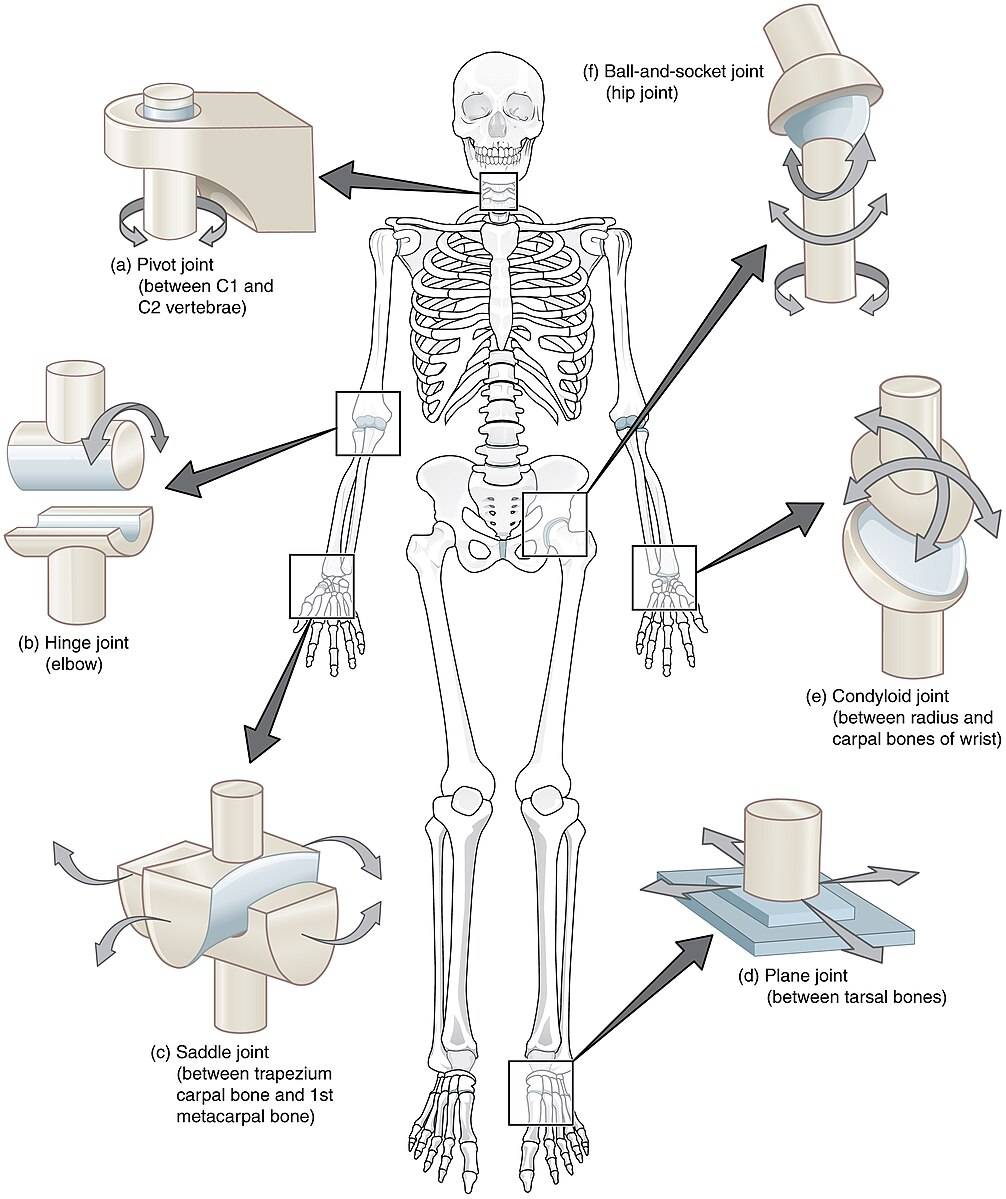
\includegraphics[width=0.6\linewidth]{files/EPpXta8zJdzN048lz8AR-c7ef96476cd11e6b82f19c58572535f8.png}
\caption[]{Image credit: OpenStax College, CC BY 3.0, via Wikimedia Commons \href{https://upload.wikimedia.org/wikipedia/commons/e/ed/909\_Types\_of\_Synovial\_Joints.jpg}{https://upload.wikimedia.org/wikipedia/commons/e/ed/909\_Types\_of\_Synovial\_Joints.jpg}}
\label{QClq2ogUPX}
\end{figure}

Some joints only allow for movement in a single plane or around a single axis of rotation (e.g. pivot joints like those that permit head rotation), while others allow for a much larger range of motion and multiple rotation angles (e.g. ball-and-socket joints in the hip or shoulder) \citep{openStax_joints}. Knowing this information about the structure of different joints will be important for understanding how these joints move in response to muscle contractions or relaxations.

\subsection{Types of movement}

Skeletal muscles rarely work in isolation. Rather, they work in pairs and larger groups to realize complex actions like walking. While walking may seem simple, it consists of a series of movements in which different joints in the body --- including ankles, knees, and hips --- change their angles, and corresponding muscles which control these joint movements must contract and relax at different moments in the cycle \citep{musculoskeletal}. Physiologists (and related experts like biomechanical engineers) use a number of terms to describe how joint angles change and the direction of movement with respect to the body \citep{openStax_movements}. Select types of movement are summarized in Figure~\ref{quLOxq4fuy} and discussed in more detail in the following sections.

\begin{figure}[!htbp]
\centering
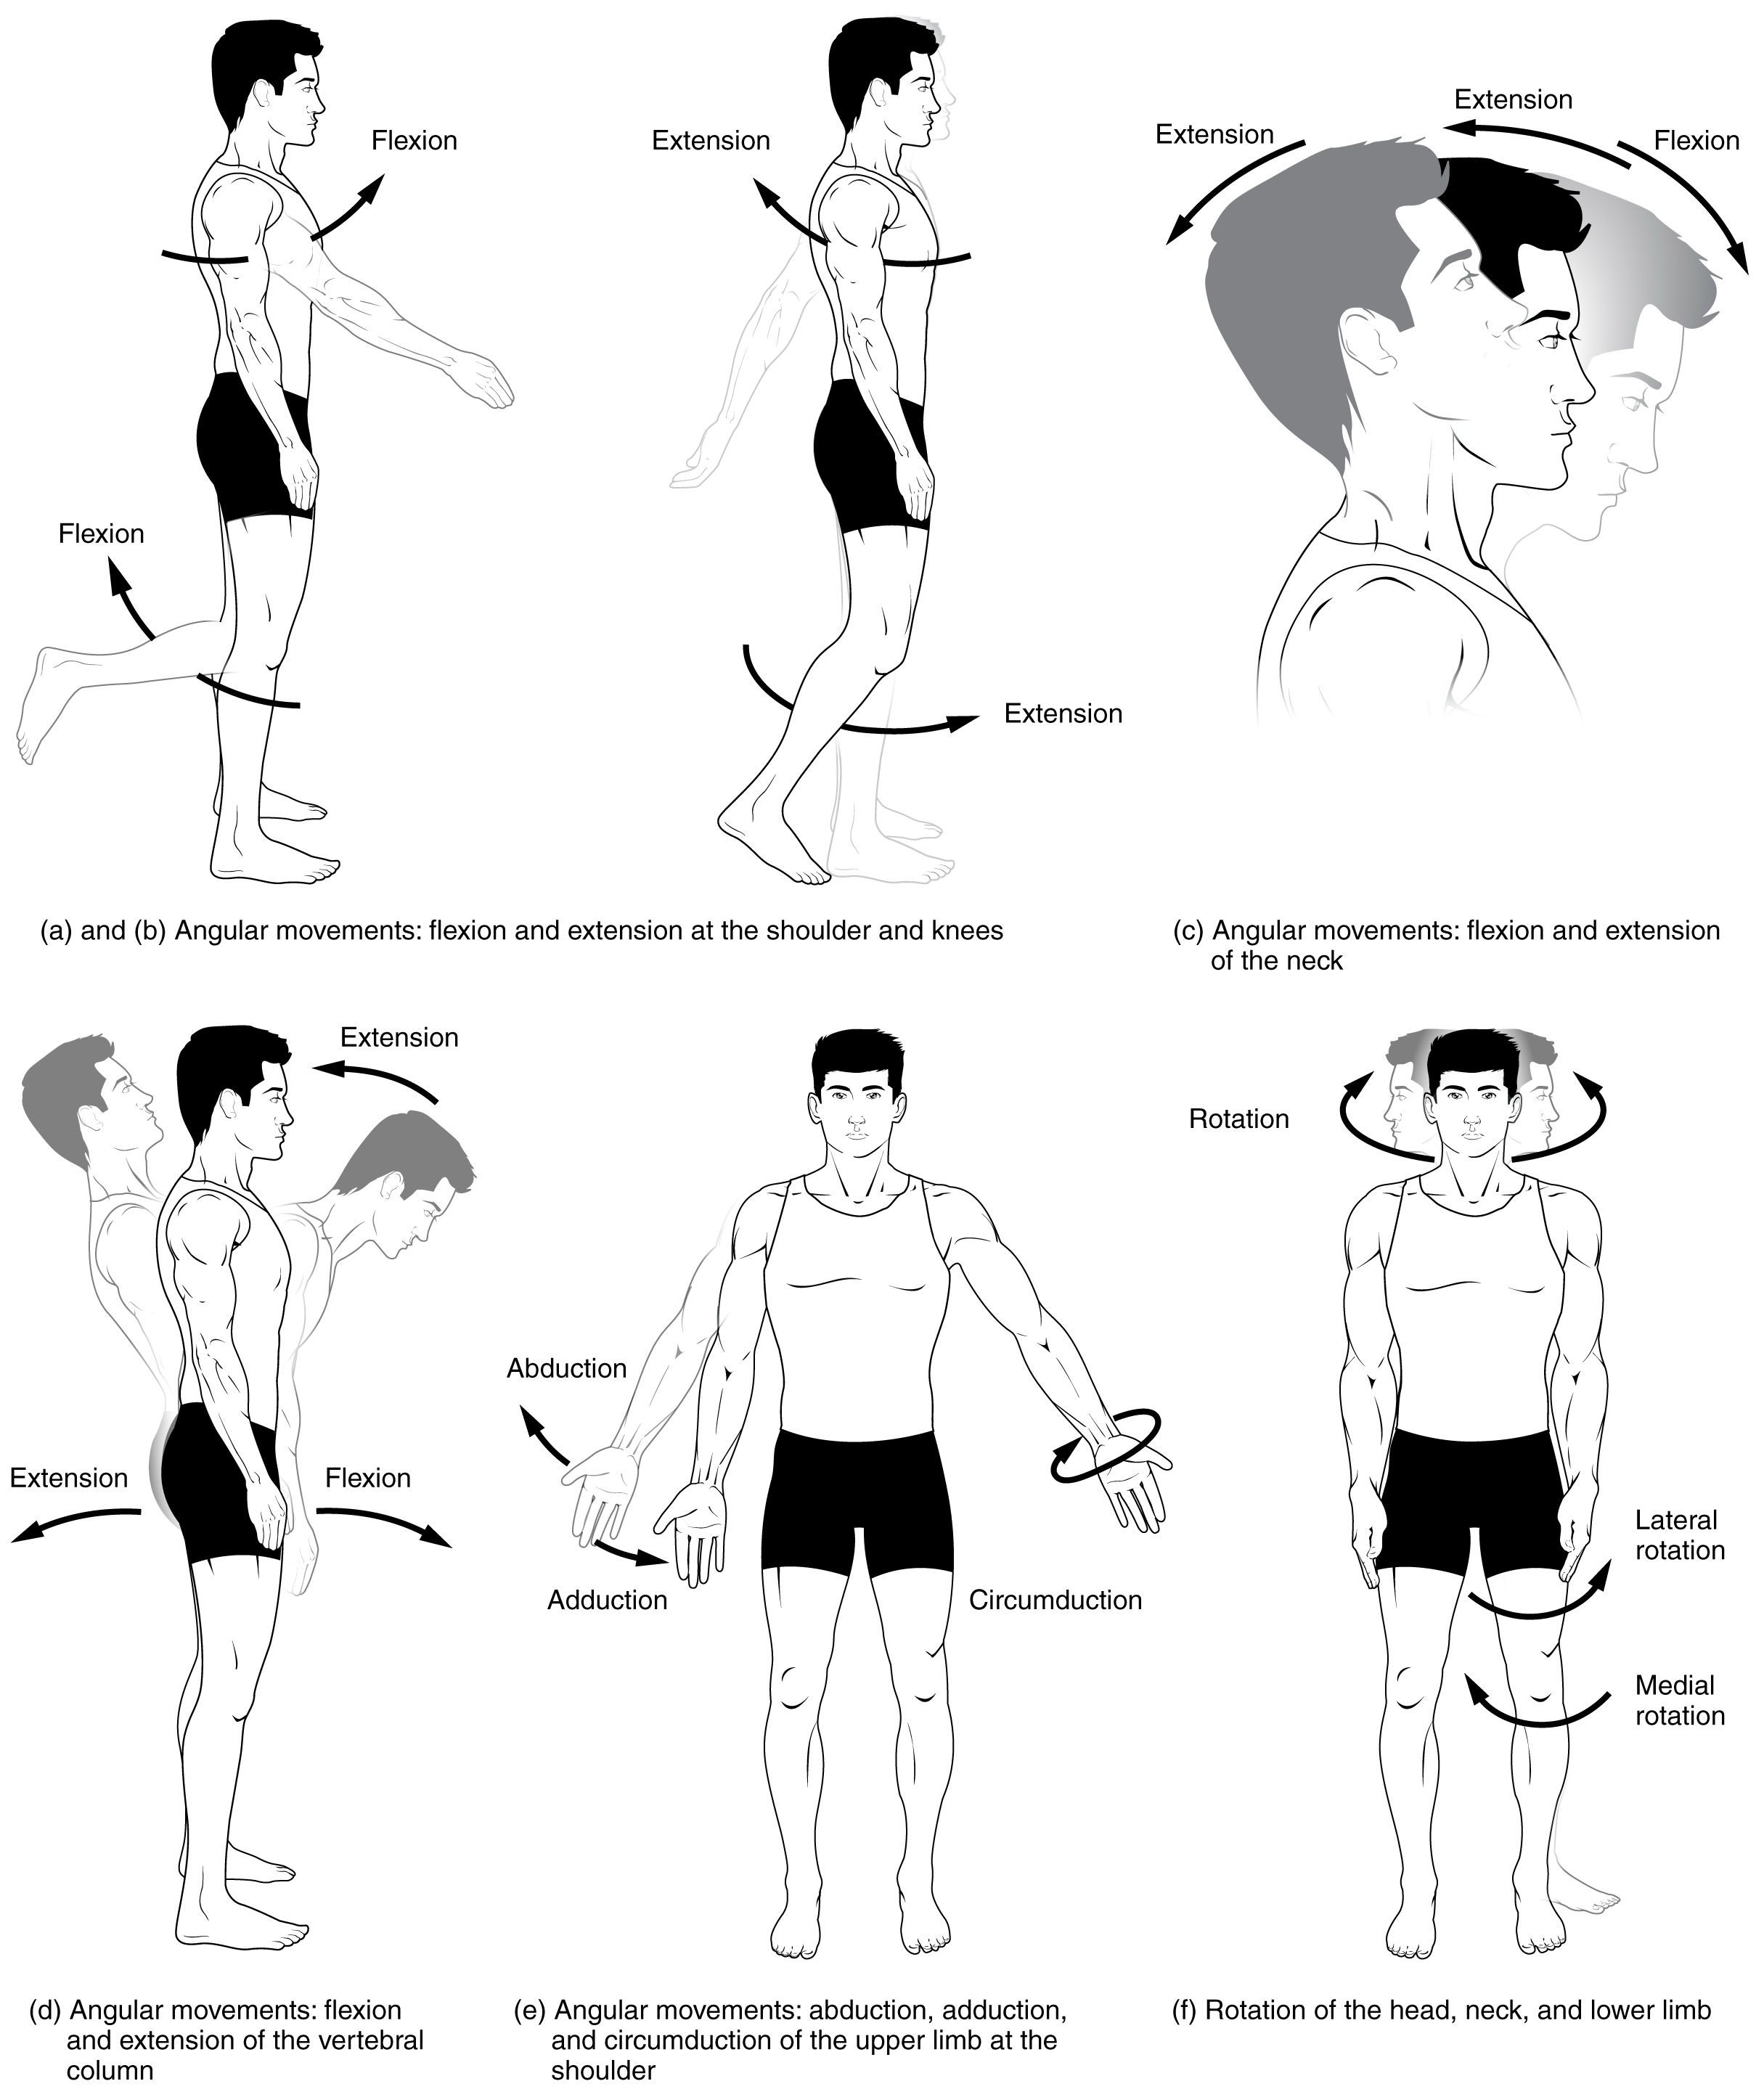
\includegraphics[width=0.7\linewidth]{files/EPpXta8zJdzN048lz8AR-865f73da41ea97aee2290807c3e391e5.png}
\caption[]{Tonye Ogele CNX, CC BY-SA 3.0, via Wikimedia Commons, \href{https://upload.wikimedia.org/wikipedia/commons/8/85/Body\_Movements\_I.jpg}{https://upload.wikimedia.org/wikipedia/commons/8/85/Body\_Movements\_I.jpg}}
\label{quLOxq4fuy}
\end{figure}

\subsubsection{Flexion and extension}

In simplest terms, flexion involves bending of the joint, while extension involves straightening (see e.g. Figure~\ref{quLOxq4fuy}a-d). Flexion and extension occurs in several joint types, including ball-and-socket, condyloid, hinge, and saddle joints \citep{openStax_movements}. For many extremities, like the fingers, arms, and legs, full extension is when the joint is at a 180\textsuperscript{o} angle, though some texts will refer to this neutral position as 0\textsuperscript{o}. Flexion begins when the joint angle decreases, with the final angle at full flexion depending on the joint in question. Extension begins again when the limb moves in the opposite direction and the joint angle increases. Many actions, like walking or repeated bicep curls, involve sequential cycles of flexion and extension \citep{}Figure \%s ``.

\begin{figure}[!htbp]
\centering
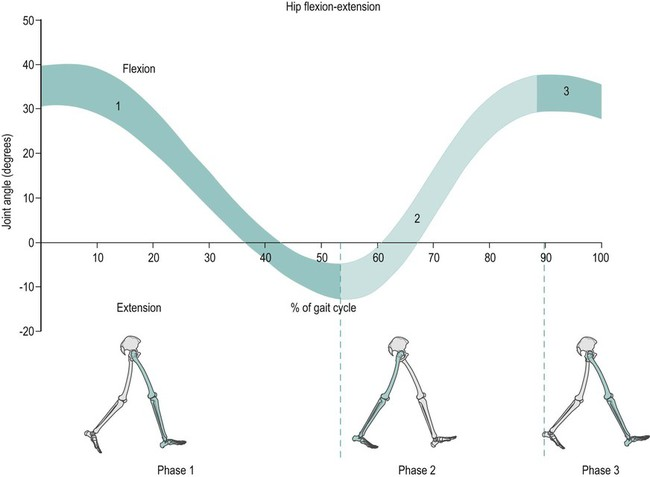
\includegraphics[width=0.8\linewidth]{files/EPpXta8zJdzN048lz8AR-8071555d61a8c30630693b2900e84506.png}
\caption[]{Hip movements and corresponding joint angles during the different phases of walking. The limb highlighted in the blue-green color is the one being tracked. Neutral position of the hip joint is considered to be 0\textsuperscript{o}, flexion is a positive value, while extension is a negative value. Image credit: Musculoskeletal Key \href{https://musculoskeletalkey.com/biomechanics-2/}{https://musculoskeletalkey.com/biomechanics-2/}}
\label{iKYfFOGvoB}
\end{figure}

In some joints, flexion and extension is less intuitive than bending a knee or elbow. Depending on the type of joint and its full range of motion (as seen in Figure~\ref{QClq2ogUPX}), there may be different ways that the joint angle can open or close. For example, the shoulder being a ball and socket joint with multiple angles of rotation means that the joint can extend or flex in both the vertical and horizontal directions \citep{cardoso2023activity}. Select muscles participate differently in these movements. Therefore, care should be taken to correctly place electrodes depending on the joint and movements to be studied.

\subsubsection{Abduction and adduction}

Ball-and-socket, condyloid, and saddle joints, but not hinge joints, can also perform opposing movements called abduction and adduction (see Figure~\ref{quLOxq4fuy}e). In loose terms, abduction refers to moving away, while adduction describes moving toward, though the point of reference for movement is different depending on whether we refer to large limbs like arms and legs, or smaller extremities like fingers \citep{openStax_movements}. In large limbs, the reference point is the midline of the body. For example, abduction of the arm (or more specifically, the shoulder joint) involves lifting the arm laterally away from the torso, while adduction involves lowering the arm back into resting position alongside the torso. For the fingers, abduction means moving the fingers away from one another, e.g. spreading all the fingers or moving a single finger laterally outward, and adduction means bringing them back together \citep{}Figure \%s ``. With the thumb, abduction involves moving the digit away from the palm and adduction means bringing the thumb back towards the palm, but these actions can happen in the radial and palmar planes. Angles for abduction and adduction will depend on the joint. For example, the thumb can abduct out to an average of around 50\textsuperscript{o}, while other digits typically reach maximums of 20-30\textsuperscript{o}\citep{erdogan2023evaluation}.

\begin{figure}[!htbp]
\centering
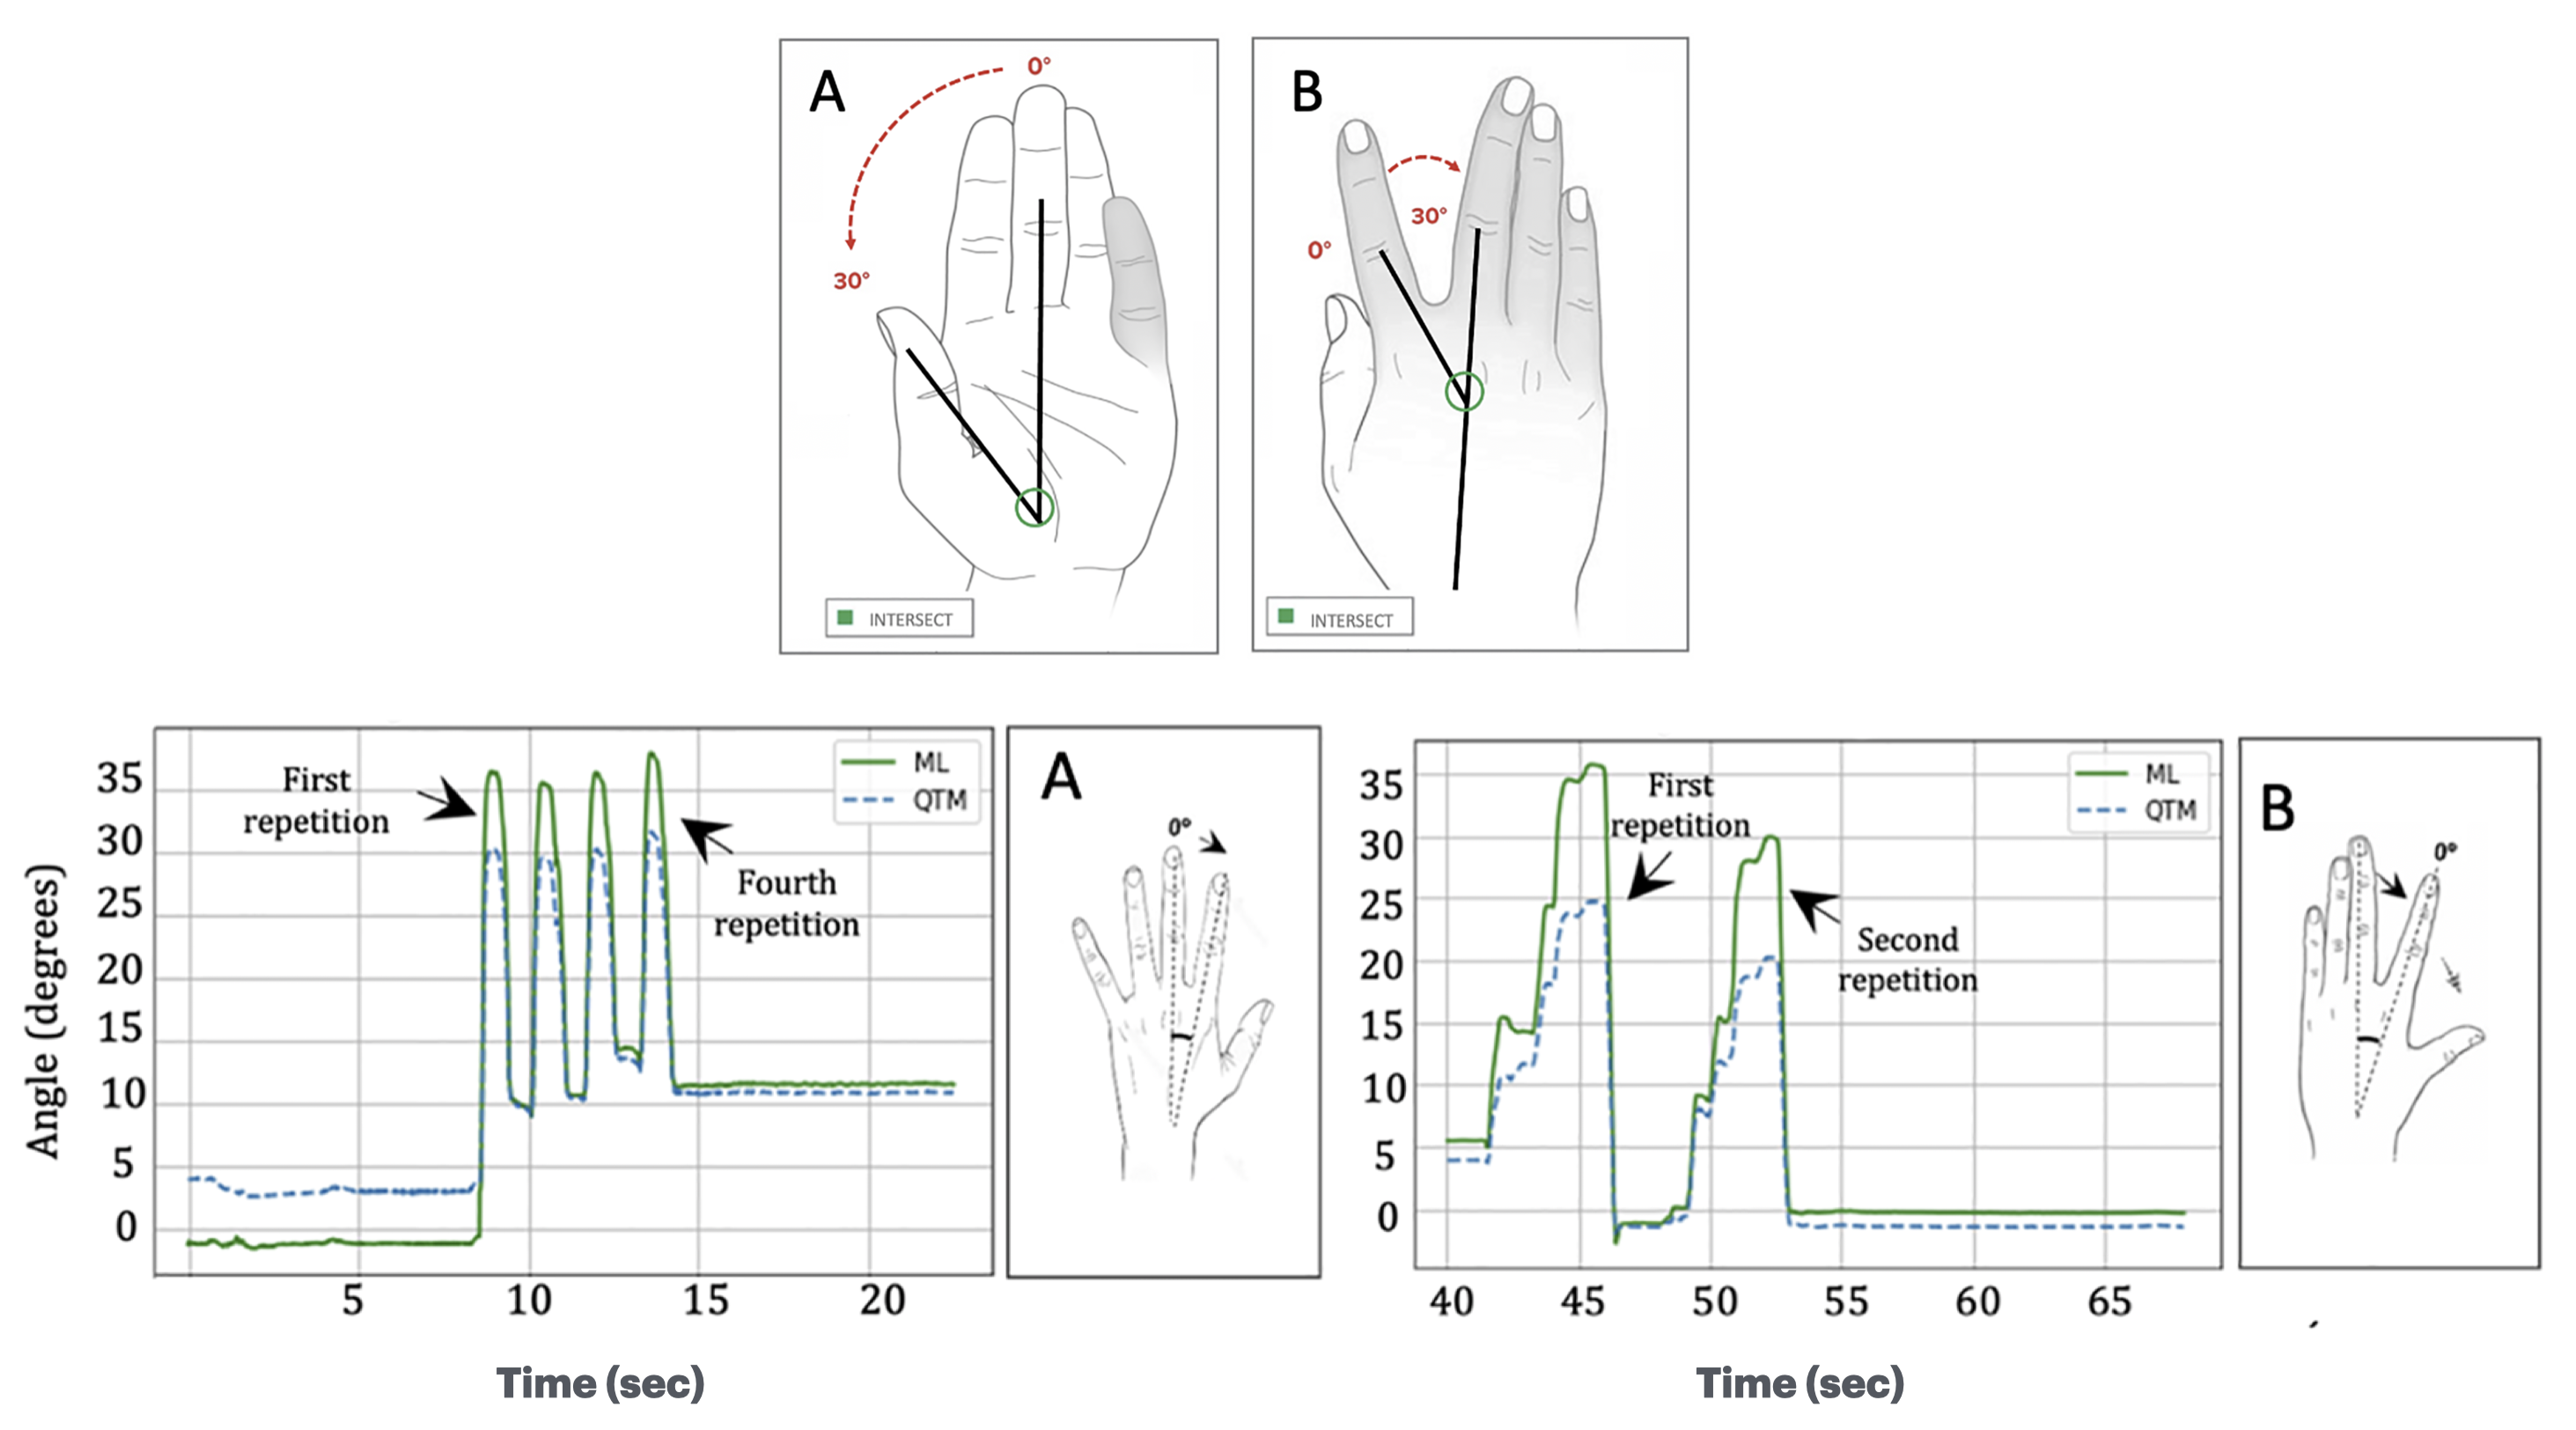
\includegraphics[width=1\linewidth]{files/EPpXta8zJdzN048lz8AR-56b271d00530c6720d8637c241e0d72b.png}
\caption[]{Image credit: Modified from \cite{Gionfrida_2022} under the terms of the CC BY license.}
\label{BVSYO3GkY2}
\end{figure}

\subsubsection{Elevation and depression}

As the terms indicate, elevation is an upward movement, while depression is downward \citep{openStax_movements}. These movements occur in the vertical (coronal) plane and only in a limited number of joints. One example is the elevation and depression involved in a shoulder shrug. While this movement may seem simple, it involves the participation of multiple joints, including the sternoclavicular (SC). acromioclavicular (AC), and scapulothoracic (ST) joints \citep{dvir1978shoulder}. In contrast to movements like flexion/extension or abduction/adduction, the elevation-opposing movement of depression may not always require active muscle contraction. In the case of shoulder depression, a good portion of the movement is due to relaxation of the upper trapezius and downward movement due to gravity \citep{cowan2023back}. However, some muscles (lower trapezius, pectoralis muscles, etc.) may engage, especially if moving the shoulder down beyond the relaxed level. If and when these muscles activate will be important for. understanding what might happen with their electrical signals measured via EMG.

\subsubsection{Study questions}

\begin{enumerate}
\item What other types of opposing movements occur in the human body? Name and briefly describe each.
\item What would be another example of elevation/depression in the human body? Which joint(s) and muscles are involved and how might you record their activity?
\item Will you be able to record any and all muscles involved in flexion/extension, abduction/adduction, or elevation/depression? Why or why not? What might be some limiting factors?
\end{enumerate}

\subsection{Muscle pairs}

\subsubsection{Agonists and antagonists}

Opposing movements like flexion and extension are accomplished by agonist and antagonist muscles, known collectively as antagonistic pairs \citep{tortora2018principles}. The classic example of such a pair includes the biceps and triceps muscles. However, which muscle is labelled the agonist or antagonist will depend on the movement being studied \citep{openStax_lever}. The agonist is also called the `primer mover', meaning it is the primary muscle involved in carrying out a specific action. So, the biceps brachii is the prime mover or agonist when examining flexion of the arm, while the triceps brachii fulfills that role in extension \citep{}Figure \%s ``. If we perform repeated biceps curls, lifting and lowering a weight, we will see alternating cycles of contraction and relaxation in the two muscles.

\begin{figure}[!htbp]
\centering
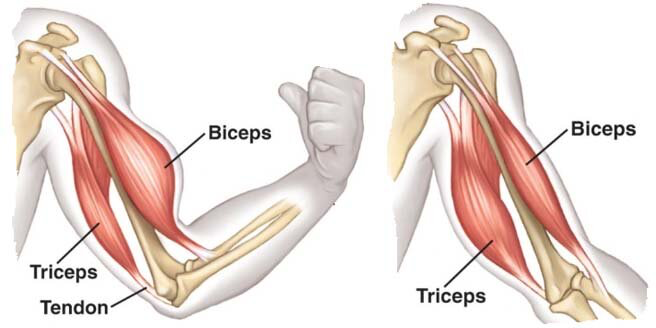
\includegraphics[width=0.7\linewidth]{files/EPpXta8zJdzN048lz8AR-ec2526a5cac2199f7f2eea233f76c576.png}
\caption[]{The biceps shortens or contracts and the triceps lengthens or relaxes during arm flexion (left). The triceps shortens or contracts and the biceps lengthens or relaxes during arm extension (right). Image source: Tudor \& Deaconescu \href{https://www.researchgate.net/figure/Agonist-antagonist-operation-of-the-biceps-and-triceps\_fig2\_326597252}{https://www.researchgate.net/figure/Agonist-antagonist-operation-of-the-biceps-and-triceps\_fig2\_326597252}}
\label{oxikRm83EQ}
\end{figure}

\subsubsection{Study questions}

\begin{enumerate}
\item Which other muscles are considered antagonistic pairs? Create a table listing the muscle names, their functions, and which acts as the agonist or antagonist in each case.
\item Will you be able to record EMGs from all the antagonistic pairs listed in exercise 1? What might be some limiting factors?
\end{enumerate}

\subsubsection{Synergists}

Instead of opposing each others actions, some muscles work together. These synergists can act to stabilize a joint to ensure that movement happens only in the desired direction \citep{openStax_lever, tortora2018principles}. Or, synergists can also aid in the contraction itself by providing additional force. Continuing with the same example as above --- arm flexion --- the agonist is often considered the biceps brachii, while the brachialis and brachioradialis are designated as synergists \citep{}Figure \%s ``.

\begin{figure}[!htbp]
\centering
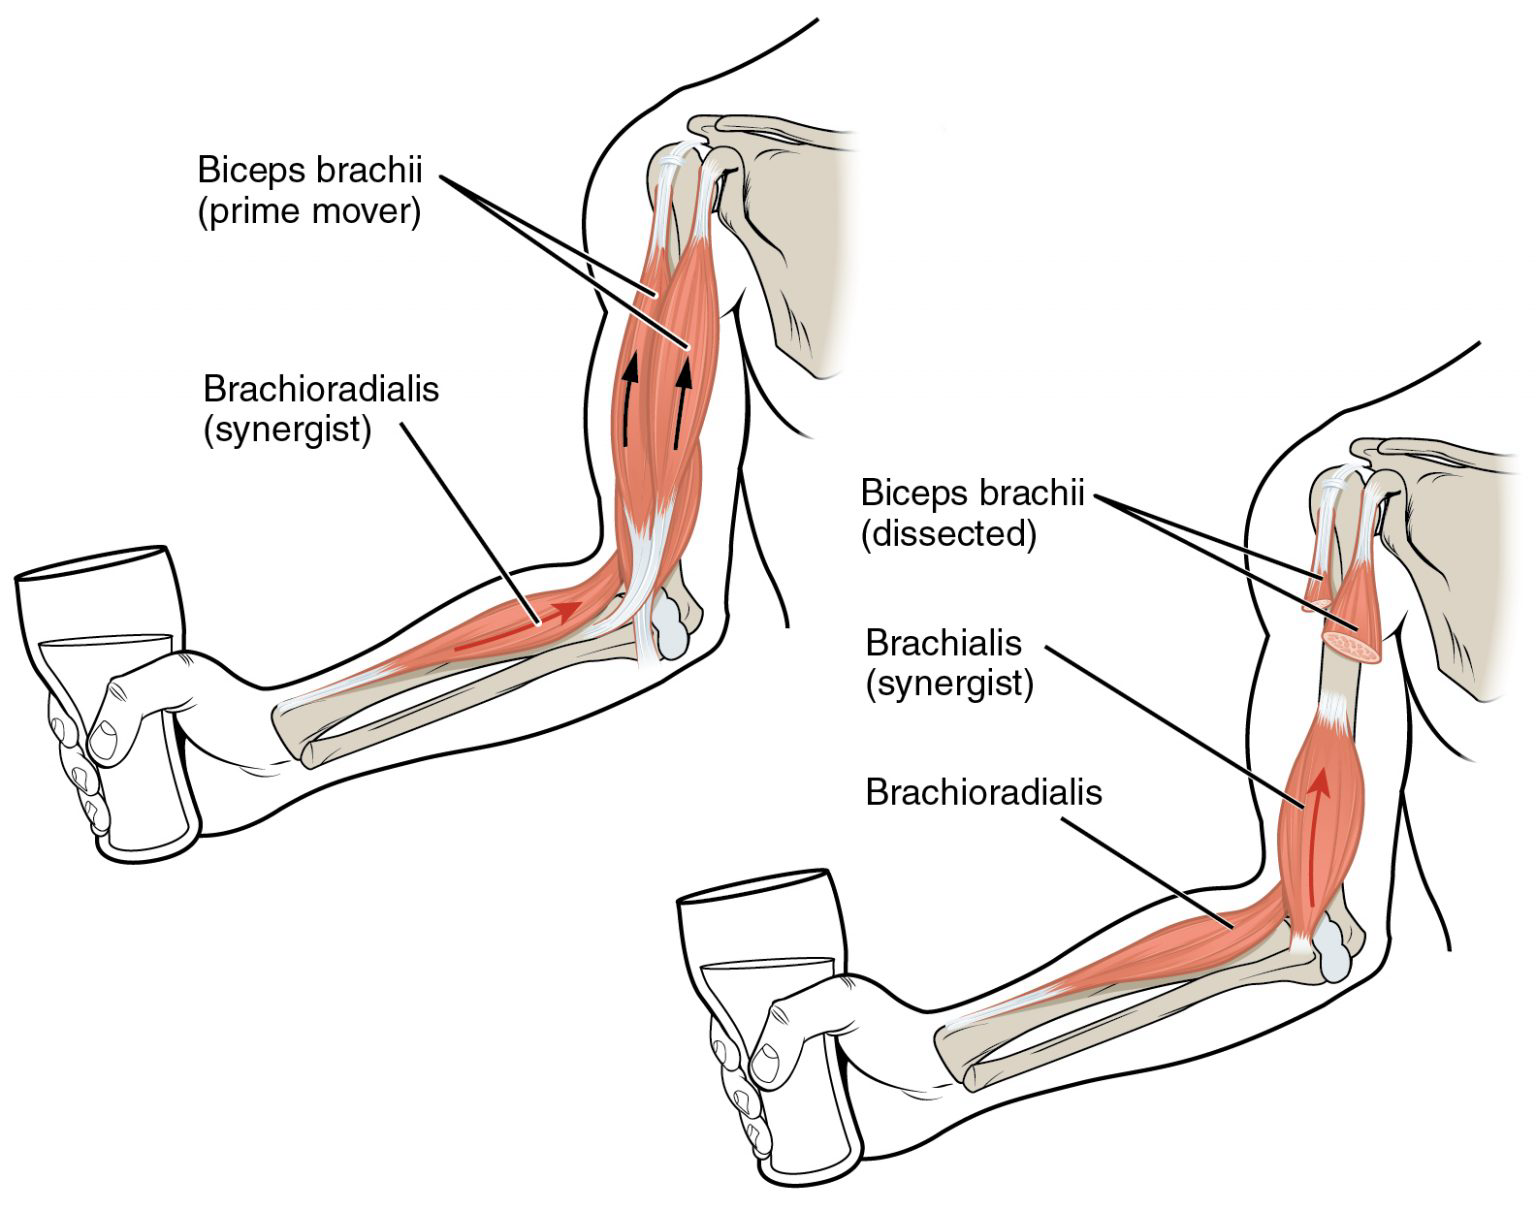
\includegraphics[width=0.7\linewidth]{files/EPpXta8zJdzN048lz8AR-fd03158f8f707eff2762e4286dda7de0.png}
\caption[]{Prime mover and synergists shown with full set of muscles (left) and with biceps dissected out to show muscles below. Image source: OpenStax College, CC BY-SA 3.0, via Wikimedia Commons \href{https://upload.wikimedia.org/wikipedia/commons/9/96/Biceps\_Muscle\_CNX.jpg}{https://upload.wikimedia.org/wikipedia/commons/9/96/Biceps\_Muscle\_CNX.jpg}}
\label{lnZL7Lff4l}
\end{figure}

Interestingly, in other references, the brachialis muscle is labelled as the primary mover for arm flexion, since it generates significantly more force during this action than the biceps. However, the relative contribution of the two muscles can depend on the position of the forearm during movement. The biceps may contribute less force during flexion if the forearm is pronated (palm of the hand facing downward) but more force if it is supinated (face upward) \citep{mansfield2019structure, plantz2023back}. Could you test this in your EMG experiments?

\section{Experimental protocol}

\subsection{Set up the dual EMG recording}

\begin{enumerate}
\item Place two surface electrodes over the bicep muscle, in parallel with the muscle fibers, and one on the back of the hand or wrist to serve as the reference/ground
\item Place another two surface electrodes over the tricep muscle in parallel with the muscle fibers; you can use the reference electrode already on the back of the hand as a common ground
\item If working with a dual channel SpikerBox (Muscle SpikerBox Pro or the Human SpikerBox), attach two red clips from one of the orange cables to the electrodes over one muscle, and then do the same with the other muscle; both black clips can be connected to the same ground electrode; connect the two orange cables to their corresponding ports on the SpikerBox \citep{}Figure \%s ``
\item If using two separate Muscle SpikerBoxes with only one channel each, carry out the steps in stage 1 and 2 of the \href{https://curvenote.com/oxa:EPpXta8zJdzN048lz8AR/hZTnTYzQR5EQmCKX51Wj}{Ch. 1: Muscle physiology and EMG basics }experimental protocol to set up the recording devices; you will need two separate phones and two people to press record at the same instant so that the recordings from the two muscles can later be synced (only do if equipment in bullet 3 is not available)
\end{enumerate}

\begin{figure}[!htbp]
\centering
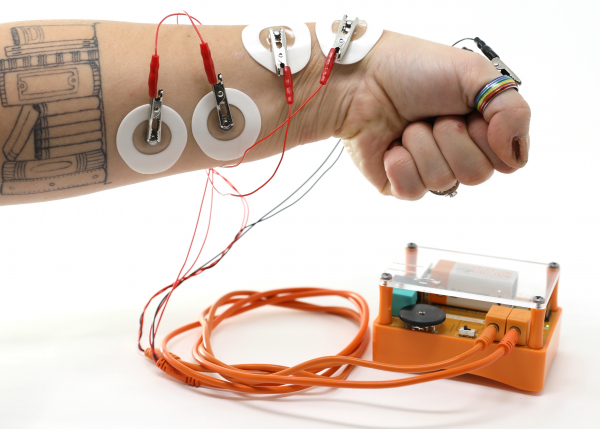
\includegraphics[width=0.7\linewidth]{files/EPpXta8zJdzN048lz8AR-fc83ca701ef50e48111b5eca101c05b6.png}
\caption[]{Human SpikerBox from Backyard Brains showing a dual muscle recording. Note that in this case, the volunteer has used their metal ring as a ground instead of a round electrode. Image credit: \href{https://backyardbrains.com/products/human-spikerbox}{https://backyardbrains.com/products/human-spikerbox}}
\label{oI7Gxpn4ek}
\end{figure}

\subsection{Studying flexion and extension}

\begin{enumerate}
\item Ask the volunteer to stand or sit such that their arm can move freely and is either hanging or resting in a relaxed position; if sitting, make sure arm can extend out fully without being impeded by the chair
\item Begin by asking the subject to flex and extend their am without any weight, and record the two EMG signals; describe what you see in terms of the activation of the bicep and tricep as the arm moves
\item Repeat the flexion and extension a few times during the recording, and then try varying the force applied to the muscles, the maximum angles of the joints, and the speed of the movements
\item Now give the subject a barbell (ideal weight will depend on the volunteer's strength); ask the volunteer to lift the weight by flexing and then lower the weight by extending their arm; describe how this compares to the muscle activation you saw for points 2 and 3
\item Again, repeat the activity a few times during the recording, and then try varying the maximum angles of the joints, the speed of the movements, and the weight used
\item Repeat this protocol but now for a different movement is which the triceps acts as the prime mover/agonist and the biceps is the antagonist
\item Repeat this protocol for muscle pairs other than the biceps and triceps; think about where else in the body you could study flexion and extension, and where you will need to place the electrodes
\end{enumerate}

\subsection{Studying abduction and adduction}

\begin{enumerate}
\item Repeat the general steps in Section~\ref{UmjcfszrGT} to set up the recordings, but now for finger abductor (dorsal interossei) and adductor (palmar interoosei) muscles
\item Place two surface electrodes on the dorsal muscle and two on the palmar muscles, with the exact location depending on which finger or digit is being studied. Because of the size of the muscles and small areas, use tab electrodes that can be cut to size
\item Place a common ground electrode on the wrist, and attach all clips as in Section~\ref{UmjcfszrGT}
\item Repeatedly move the digit of interest away from the midline (abduction) and back toward the midline (adduction)
\item Try varying the force, moving the finger slowly outward or slowly inward and then holding at the maximum position for several seconds
\item Compare the recording when moving the finger in the horizontal plane versus moving it vertically, i.e. lifting the finger up and down
\item Compare the recording when moving the finger actively (performing a contraction) versus passively, i.e. using another finger to displace the finger of interest while not contracting
\end{enumerate}

\subsection{Studying elevation and depression}

\begin{enumerate}
\item Repeat the general steps in Section~\ref{UmjcfszrGT} to set up the recordings, but now for mandibular muscles controlling elevation (masseter) and depression (lateral pterygoid)
\item Place two surface electrodes on the masseter (vertical placement) and two on the lateral pterygoid (horizontal placement). Because of the size of the muscles and small areas, use smaller round electrodes, e.g. pediatric size (40mm diameter)
\item Place a common ground electrode over the mastoid process behind the ear, and attach all clips as in Section~\ref{UmjcfszrGT}
\item Repeatedly open (depress) and close (elevate) the jaw
\item Try varying the force, opening and closing the jaw slowly and then holding at the maximum open or clenched position for several seconds
\item Compare the recording when performing elevation and depression versus other actions like chewing or smiling
\end{enumerate}

\clearpage
\bibliography{main.bib}

\end{document}
